\chapter{Komponententaxonomie und Metamodell (MB.OS Vans)}\label{chap:metamodell}

\noindent
Dieses Kapitel entwickelt eine erweiterbare Komponententaxonomie und ein präzises Metamodell für eine moderne, dienstorientierte E/E-Architektur im Sinne von MB.OS (Fokus: Vans). Es adressiert eine zonale Topologie mit zentralen Rechenknoten, Ethernet-Backbone (TSN), serviceorientierter Kommunikation, sicherheitskritischen Funktionsketten und domänenspezifischer Sensorik/Aktorik für Nutzfahrzeug-typische Use-Cases (z.\,B. Lieferlogistik, leichte Nutzfahrzeuge, Flottenbetrieb).

\section{Grundprinzipien und Struktur}
\subsection{Zonale Architektur und zentrale Rechenplattform}
\begin{itemize}
  \item \textbf{Zonen-Controller (ZC)}: Versorgungs- und IO-Nähe, Aggregation lokaler Sensorik/Aktorik, Vorverarbeitung.
  \item \textbf{Zentrale Rechenplattform (Central Compute, CC)}: Hochperformant (CPU/GPU/NPU), Safety-Partitionen (ASIL) und Virtualisierung.
  \item \textbf{Ethernet-Backbone mit TSN}: Deterministische Latenzen, Priorisierungen, Redundanzen.
  \item \textbf{Serviceorientierung}: DDS/SOME\-IP für verteilte Dienste, Versionierung, QoS.
\end{itemize}

\subsection{Domänen und Use-Cases (Vans)}
Karosserie/Body, Antrieb/Powertrain, Fahrerassistenz/AD, Infotainment/HMI, Fracht-/Laderaumdomäne (z.\,B. Kühlung, Zustelllogik), Flotten-/Telematikdienste (OTA, Diagnose, Fleet Operations).

\section{Komponententypen (Taxonomie)}
\subsection{Rechenknoten}
\begin{itemize}
  \item \textbf{AD Domain Controller (AD-DC)}: Perzeption, Fusion, Planung, Regelung; GPU/NPU-beschleunigt.
  \item \textbf{Zonen-ECU (ZC)}: IO-Management, Aktorik/Sensorik, lokale Diagnosen; Gateways zu CAN/LIN.
  \item \textbf{Gateway/Switch} (L3/L2, TSN-fähig): Segmentierung, Redundanzpfade, Traffic Shaping.
  \item \textbf{Telematik/Connectivity ECU (TCU)}: 5G/LTE, WLAN, GNSS; OTA, Flottenintegration.
  \item \textbf{HMI/Infotainment ECU}: Anzeige/Bedienung, Audio/Video, Interaktion.
\end{itemize}

\subsection{Sensorik}
Kameras (Mono/Stereo/Surround), Radar (Kurz-/Mittel-/Langstrecke), LiDAR, Ultraschall, GNSS/IMU, Fracht-/Laderaumsensorik (Temperatur, Türkontakte, Gewicht, Kamera), Innenraumkameras.

\subsection{Aktorik}
Lenkung (EPS), Bremse (EHB/EMB), Antrieb, Fahrwerk/Dämpfer, Lichtsysteme, Türen/Heckklappen, Laderaumklima.

\subsection{Kommunikation}
Ethernet (1/2.5/10 GbE) mit TSN (Zeitsynchronisation, Scheduling, Shaping), CAN/CAN-FD, LIN; ggf. FlexRay (Legacy); DDS/SOME\-IP auf Service-Ebene.

\subsection{Infrastruktur}
Switches, Power Distribution Units, Speicher/Storage, Sicherheitsmodule (HSM/TPM), Takt-/Zeitquellen.

\section{Metamodell-Elemente}
\subsection{Strukturale Basisklassen}
\noindent
\textbf{Node}, \textbf{Port}, \textbf{Interface}, \textbf{Link}, \textbf{NetworkSegment}; \textbf{PowerDomain}, \textbf{TimingDomain}.

\subsection{Kommunikationsartefakte}
\noindent
\textbf{Message}, \textbf{Signal}, \textbf{TrafficFlow}, \textbf{Service}, \textbf{Topic}; \textbf{QoSProfile} (Periodizität, Deadline, Latenzbudget, Priorität, Zuverlässigkeit), \textbf{TSNSchedule}.

\subsection{Software-/Laufzeitelemente}
\noindent
\textbf{SoftwareComponent (SWC)}, \textbf{Task}, \textbf{Runnable}, \textbf{Chain}; \textbf{SchedulingPolicy} (preemptive/fixed priority/TSN-triggered), \textbf{WCET/BCET}.

\subsection{Deployment und Safety}
\noindent
\textbf{Deployment}, \textbf{Partition}, \textbf{RedundancyGroup}, \textbf{ASILLevel}, \textbf{HealthMonitor}, \textbf{DiagnosticFunction}.

\subsection{Ressourcen- und Energiedaten}
\noindent
\textbf{ComputeProfile} (CPU/GPU/NPU-Kapazität), \textbf{MemoryProfile}, \textbf{StorageProfile}, \textbf{PowerStateModel} (Duty-Cycle, Übergangszeiten), \textbf{ThermalEnvelope}.

\section{Attributkatalog (Auszug)}
\begin{table}[h]
  \centering
  \caption{Rechenknoten-Attribute (Auszug)}
  \begin{tabular}{lll}
    \toprule
    Attribut & Typ & Beschreibung \\
    \midrule
    cpu\_cores & Integer & Anzahl/Topologie (big.LITTLE) \\
    gpu\_tflops & Float & Rechenleistung GPU/NPU \\
    virtualization & Enum & none | hypervisor | containers \\
    asil\_level & Enum & QM | A | B | C | D \\
    power\_states & List & Zustände + Übergangszeiten \\
    thermal\_max & Float & zulässige Verlustleistung (W) \\
    \bottomrule
  \end{tabular}
\end{table}

\begin{table}[h]
  \centering
  \caption{Kommunikations-Attribute (Auszug)}
  \begin{tabular}{lll}
    \toprule
    Attribut & Typ & Beschreibung \\
    \midrule
    link\_speed & Enum & 100M | 1G | 2.5G | 10G \\
    tsn\_prio & Integer & 0..7 (IEEE 802.1Q) \\
    latency\_budget & Float & Ziel-Latenz (ms) \\
    jitter\_budget & Float & Ziel-Jitter (ms) \\
    redundancy & Enum & none | PRP | HSR | dual-path \\
    \bottomrule
  \end{tabular}
\end{table}

\section{Stereotypen und Erweiterbarkeit}
\subsection{Stereotyp-Mechanismus}
Stereotypen erweitern Basisklassen um domänenspezifische Felder (z.\,B. \emph{CameraSensor}, \emph{ADComputeNode}, \emph{TSNBackboneLink}), versioniert und validiert über Schema-Definitionen.

\subsection{Beispielhafte Stereotypen}
\begin{itemize}
  \item \textbf{CameraSensor}: fov\_h/v, resolution, framerate, compression, preprocessing\_level
  \item \textbf{RadarSensor}: bands, range, update\_rate, doppler\_resolution
  \item \textbf{LiDARSensor}: channels, spin\_rate, point\_density, range
  \item \textbf{ADComputeNode}: gpu\_tflops, npu\_tops, asil\_isolation, virtualization
  \item \textbf{TSNBackboneLink}: gate\_schedule, guard\_bands, prio\_map
\end{itemize}

\section{Zonen-Topologie (Diagramm)}
\begin{figure}[h]
  \centering
  \begin{tikzpicture}[node distance=1.2cm and 1.6cm,>=Latex]
    % Central Compute
    \node[draw,rounded corners,fill=blue!10,minimum width=4.2cm,minimum height=1.2cm] (cc) {Central Compute (AD-DC)};
    % Switch backbone
    \node[draw,rounded corners,fill=gray!15,below=1.0cm of cc,minimum width=5.0cm,minimum height=1.0cm] (sw) {TSN Ethernet Backbone (Switches)};
    % Zones
    \node[draw,rounded corners,fill=green!10,left=2.8cm of sw,minimum width=3.2cm] (zf) {Front-Zone ECU};
    \node[draw,rounded corners,fill=green!10,below left=0.6cm and -0.2cm of sw,minimum width=3.2cm] (zl) {Left-Zone ECU};
    \node[draw,rounded corners,fill=green!10,below right=0.6cm and -0.2cm of sw,minimum width=3.2cm] (zr) {Right-Zone ECU};
    \node[draw,rounded corners,fill=green!10,right=2.8cm of sw,minimum width=3.2cm] (zb) {Rear-Zone ECU};
    % Links
    \draw[->,thick] (cc) -- (sw);
    \draw[<->,thick] (sw) -- (zf);
    \draw[<->,thick] (sw) -- (zl);
    \draw[<->,thick] (sw) -- (zr);
    \draw[<->,thick] (sw) -- (zb);
    % Sensors/Actuators
    \node[draw,rounded corners,fill=yellow!20,below=0.8cm of zf,minimum width=2.6cm] (cams) {Cameras/Radar/LiDAR};
    \node[draw,rounded corners,fill=orange!20,below=0.8cm of zb,minimum width=2.6cm] (act) {Steering/Brake/Drive};
    \draw[-,thick] (zf) -- (cams);
    \draw[-,thick] (zb) -- (act);
  \end{tikzpicture}
  \caption{Zonen-Topologie mit zentraler Rechenplattform und TSN-Backbone (schematisch).}
  \label{fig:zonen_topologie}
\end{figure}

\section{Datenflussketten (Perzeption \textrightarrow{} Aktorik)}
\begin{figure}[h]
  \centering
  \begin{tikzpicture}[node distance=1.3cm,>=Latex]
    \node[draw,fill=yellow!20,rounded corners] (cam) {Kamera-Stream};
    \node[draw,fill=blue!10,rounded corners,right=2.0cm of cam] (pre) {Preprocessing (ZC)};
    \node[draw,fill=blue!20,rounded corners,right=2.2cm of pre] (perc) {Perzeption (AD-DC)};
    \node[draw,fill=blue!30,rounded corners,right=2.2cm of perc] (plan) {Planung/Regelung (AD-DC)};
    \node[draw,fill=orange!20,rounded corners,right=2.2cm of plan] (act) {Lenk-/Bremsaktor};
    \draw[->,thick] (cam) -- node[above]{Ethernet/TSN} (pre);
    \draw[->,thick] (pre) -- node[above]{DDS/SOME\-IP} (perc);
    \draw[->,thick] (perc) -- node[above]{DDS/SOME\-IP} (plan);
    \draw[->,thick] (plan) -- node[above]{CAN-FD/TSN} (act);
  \end{tikzpicture}
  \caption{Beispielhafte Ende-zu-Ende-Kette von Sensorik über zentrale Rechenfunktion zur Aktorik.}
  \label{fig:e2e_chain}
\end{figure}

\section{Qualitätsattribute und Metriken}
\subsection{Timing und Determinismus}
E2E-Latenzbudgets, Jittergrenzen, Periodizitäten, Deadline-Misses; TSN-Schedule-Integration und Priorisierungsregeln.

\subsection{Bandbreite und Auslastung}
Linkauslastung, Queuing, Shaping; Redundanzpfade; Gateway-Last und Frame-/Signal-Aggregation.

\subsection{Rechenlast und Energie}
CPU/GPU/NPU-Profilierung (WCET/BCET, Duty-Cycles), Power-State-Strategien, thermische Budgetierung.

\subsection{Safety und Security}
ASIL-gerechte Partitionierung, Freedom-from-Interference, Diagnose- und Health-Management; Secure Boot, Key-Management, Secure Onboard Communication.

\section{Validierungsregeln (Ausschnitt)}
\begin{itemize}
  \item Jeder \emph{TrafficFlow} besitzt ein \emph{QoSProfile} mit Periodizität, Deadline und Priorität.
  \item TSN-\emph{Schedule} deckt alle deterministischen Flows ohne Konflikte ab (Guard Bands, Gate States).
  \item \emph{Deployment} wahrt ASIL-Isolationsregeln; Redundanzgruppen sind physikalisch entkoppelt.
  \item \emph{PowerStateModel} ist konsistent mit Latenzanforderungen (Aufwachzeiten \(\leq\) Budget).
\end{itemize}

\section{Zusammenfassung}
Die vorgestellte Taxonomie und das Metamodell bilden eine MB.OS-nahe, zonale E/E-Architektur für Vans ab. Sie sind erweiterbar, quantitativ auswertbar und dienen als Grundlage für die Synthese-Metrik und die Transformation in Simulationsmodelle.

\newpage
\section{Fallstudie A: Zustell-Van mit Kühlkette (Urban Last Mile)}
\subsection{Ausgangslage und Anforderungen}
Ein urbaner Zustell-Van mit temperaturgeführtem Laderaum (2 Zonen), L2-Assistenz (Stop-and-Go, Spurführung), Flottenanbindung und OTA-Updates. Anforderungen: \(\text{E2E} < 100\,\text{ms}\) für Lenk-/Bremsketten, \(\pm 0.5\,\degree\text{C}\) Temperaturregelung, hochverfügbare Tür-/Sicherheitsfunktionen.

\subsection{Architekturzuordnung}
\begin{itemize}
  \item Zonen-ECUs: Front (Perzeption-Sensor-IO), Rear (Laderaum IO, Aktorik Kühlung/Heckklappe)
  \item Central Compute: AD-DC mit GPU/NPU; TSN-Backbone (1/2.5 GbE), PRP für Sicherheitsketten
  \item Services: Perception\_Detections, Planning\_Trajectory, Cargo\_TempReport, Door\_Access
\end{itemize}

\subsection{Ende-zu-Ende-Kette (Lenkung)}
\begin{table}[h]
  \centering
  \caption{E2E-Budgetzerlegung (Lenkung, urban)}
  \begin{tabular}{lll}
    \toprule
    Teilpfad & Anteil [ms] & Erläuterung \\
    \midrule
    Sensoringress (ZC) & 8 & Vorverarbeitung, Timestamping \\
    Netz (ZC $\rightarrow$ CC) & 6 & TSN, Prio Q7, 2 Hops \\
    Perzeption + Planung (CC) & 50 & GPU/NPU Pipelines \\
    Netz (CC $\rightarrow$ ZC Rear) & 6 & TSN, Gate-Window synchron \\
    Aktuatorbus (CAN-FD) & 10 & Kommandotransfer \\
    Sicherheitsmarge & 20 & Jitter/Spitzen \\
    \midrule
    Summe & 100 & innerhalb Budget \\
    \bottomrule
  \end{tabular}
\end{table}

\subsection{Energieprofil Laderaumsensorik}
Duty-Cycle-Strategie: \emph{sleep} (90\%), \emph{idle} (5\%), \emph{active} (5\%). Bei \(P_{sleep}=0.02\,\text{W}, P_{idle}=0.2\,\text{W}, P_{active}=1.0\,\text{W}\) ergibt sich \(P_{avg}=0.072\,\text{W}\). Aufwachzeit \(t_{wake}=50\,\text{ms}\) ist mit E2E-Anforderungen für Tür-/Alarmdienste verträglich (nicht sicherheitskritisch).

\newpage
\section{Fallstudie B: Regionalverkehr/Autobahn (L2+/L3-Features)}
\subsection{Ausgangslage und Anforderungen}
Langstrecke mit höheren Geschwindigkeiten: engere E2E-Budgets (Lenkung 60 ms), höhere Sensorraten (Kameras 4x60 FPS, Radar 20 Hz, LiDAR 10 Hz), verlässliche Redundanz.

\subsection{TSN-Planung und Redundanz}
\begin{itemize}
  \item TSN-GCL mit verdichteten Q7-Fenstern (alle 0.25 ms) für Perzeption/Control
  \item PRP auf Backbone, Dual-Homing der AD-DC zu zwei Switch-Bäumen
  \item DDS \emph{Perception\_Critical}: reliable, Deadline 3 ms, Latenzbudget 1 ms
\end{itemize}

\subsection{Rechenlastvariante}
\begin{table}[h]
  \centering
  \caption{Perzeptionsvariante (hohe Rate)}
  \begin{tabular}{llll}
    \toprule
    Sensor & Rate & Datenrate & Last (Tendenz) \\
    \midrule
    Kamera & 60 FPS & \SI{298}{Mbit/s} (H.265 k=50) & hoch (GPU/NPU) \\
    Radar & 20 Hz & \SI{20}{Mbit/s} & mittel (CPU) \\
    LiDAR & 10 Hz & \SI{200}{Mbit/s} & hoch (GPU) \\
    \bottomrule
  \end{tabular}
\end{table}
Optimierungen: Region-of-Interest (ROI) Vorverarbeitung am ZC, adaptive Kompression, Scheduling-Priorisierung.

\newpage
\section{Konkrete QoS-Profile und Serviceversionierung}
\subsection{QoS-Profile (DDS/SOME-IP)}
\begin{table}[h]
  \centering
  \caption{QoS-Parameter (Beispiele)}
  \begin{tabular}{lllll}
    \toprule
    Service & Reliability & History & Deadline [ms] & Latenzbudget [ms] \\
    \midrule
    Perception\_Detections & reliable & keep\_last(5) & 5 & 2 \\
    Planning\_Trajectory & reliable & keep\_last(3) & 2 & 1 \\
    Cargo\_TempReport & best-effort & keep\_last(1) & 200 & 100 \\
    Door\_Access & reliable & keep\_all & 50 & 10 \\
    \bottomrule
  \end{tabular}
\end{table}

\subsection{Versionierung/Kompatibilität}
Service-IDs und Versionsfelder (major/minor) sind Teil des Interfacevertrags; \emph{compatibility policies} (strict/relaxed) steuern Interoperabilität. Deployment-Regeln verlangen koexistente Minor-Versionen bei Rolling Updates (OTA).

\newpage
\section{TSN-Engineering: Von Anforderungen zur GCL}
\subsection{Anforderungsableitung}
Aus E2E-Forderungen werden Flow-spezifische Budgets abgeleitet: \(B_{net}=\{1..8\}\,\text{ms}\) je Kette. Daraus ergeben sich Queue-Prioritäten und Gate-Fenstergröße. 

\subsection{Beispiel-GCL Ableitung}
Bei \(T_{cycle}=1\,\text{ms}\) und kritischem Flow mit \(L_{net}=200\,\mu s\) wird \(\geq 0.25\,\text{ms}\) Gate-Zeit für Q7 reserviert; Guard Band 0.05 ms. Übrige Zeit an Q6/Q5 (Diagnose/HMI) und Q0..Q4 (Best-Effort).

\newpage
\section{Sicherheits- und Diagnosepfade (ASIL, Health-Monitoring)}
\subsection{ASIL-Isolation}
Safety-relevante SWCs laufen in isolierten Partitionen/VMs; Zugriff auf Bus/Netz via geprüften Proxies (Freedom from Interference). 

\subsection{Health-Monitoring}
Watchdogs, Heartbeats und Thresholds (z.\,B. Max Jitter, Paketverlust) lösen Degradationsmodi aus (Fallback-Sensorik, niedrigere Feature-Stufe), stillhalten gemäß \cite{iso26262}.

\newpage
\section{Gateway-Strategien: Aggregation, Routing, Security}
\subsection{Aggregation}
Signale mit gleicher Periodizität und Ziel werden zu Frames/Flows gebündelt; reduziert Overhead und Jitter, erfordert dafür Framegrößen-/Maximum Transmission Unit (MTU)-Anpassung.

\subsection{Routing}
Statische Pfade für deterministische Ketten; dynamische Pfade (ECMP) für non-critical Services. PRP-/HSR-Pfade sind entkoppelt von Best-Effort.

\subsection{Security}
Message Authentication (MAC), Secure Onboard Communication, Firewall-Regeln und Service-ACLs schützen gegen unautorisierte Zugriffe.

\newpage
\section{Detaillierte Stereotypen-Beispiele}
\subsection{CameraSensor}
Attribute: \emph{fov\_h/v, resolution, framerate, compression, preprocessing\_level, thermal\_range}. Beispiel: Front-Kamera 120°/70°, 1920x1080 @60FPS, H.265 k=50, preprocessing=low.

\subsection{ADComputeNode}
Attribute: \emph{gpu\_tflops, npu\_tops, asil\_isolation, virtualization, thermal\_max}. Beispiel: 30 TFLOPS, 120 TOPS, ASIL-VM, Hypervisor, 80 W.

\subsection{TSNBackboneLink}
Attribute: \emph{gate\_schedule, guard\_bands, prio\_map, redundancy}. Beispiel: GCL-Zyklus 1 ms, Q7 0.25 ms, Guard 0.05 ms, PRP.

\newpage
\section{Traceability: Von Anforderung zu Modell und Simulation}
\begin{itemize}
  \item Anforderung \(\rightarrow\) Modellattribute (QoS, Latenzbudget, ASIL)
  \item Modellattribute \(\rightarrow\) GCL/Deployment/Mapping-Regeln
  \item Regeln \(\rightarrow\) Simulationsartefakte (Flows, Schedules, Tasks)
\end{itemize}
Diese Rückverfolgbarkeit ermöglicht gezieltes Varianten- und What-if-Engineering.
\section{Use-Cases und Domänenspezifika für Vans}
\subsection{Flotten- und Zustelllogistik}
Routenoptimierung, vorausschauende Wartung, dynamische Ladungsüberwachung (Temperatur, Gewicht, Türzustände), Just-in-Time-Lieferfenster. Erfordert robuste Konnektivität (5G/DSRC/WLAN), sichere OTA-Mechanismen und priorisierte Datenkanäle.

\subsection{Laderaumdomäne}
Kühlkettenmanagement, Videoüberwachung, Zutrittskontrolle, Telematik-Integration. Hohe Sensordichte, teils batteriebetriebene Geräte, energieeffiziente Kommunikationsmodi (Wake-on-LAN, Low-Power-States).

\subsection{Assistiertes/Automatisiertes Fahren (L2/L3)}
Perzeption (Kamera/Radar/LiDAR), Fusion, Lokalisierung, Pfadplanung, Aktorik. Strenge Latenz- und Safety-Anforderungen \cite{iso26262,ieee8021q}.

\newpage
\section{TSN-Scheduling-Beispiel (Zeitgating)}
\begin{figure}[h]
  \centering
  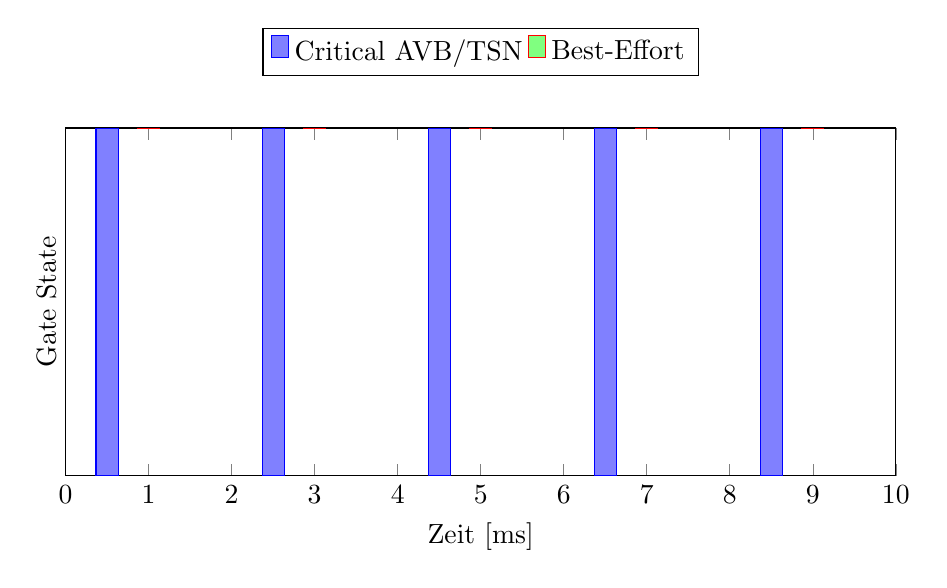
\begin{tikzpicture}
    \begin{axis}[
      ybar stacked,
      width=\textwidth,
      height=6cm,
      ylabel={Gate State},
      xlabel={Zeit [ms]},
      xmin=0, xmax=10,
      ymin=0, ymax=1,
      ytick=\empty,
      legend style={at={(0.5,1.15)},anchor=south,legend columns=-1},
      bar width=8pt
    ]
      \addplot+[ybar,fill=blue!50] coordinates {(0.5,1) (2.5,1) (4.5,1) (6.5,1) (8.5,1)}; \addlegendentry{Critical AVB/TSN}
      \addplot+[ybar,fill=green!50] coordinates {(1.0,1) (3.0,1) (5.0,1) (7.0,1) (9.0,1)}; \addlegendentry{Best-Effort}
    \end{axis}
  \end{tikzpicture}
  \caption{Schema eines wiederkehrenden TSN-Gate-Schedules (vereinfachte Visualisierung, vgl. \cite{ieee8021q}).}
  \label{fig:tsn_gating}
\end{figure}

\noindent
Der Gate-Plan unterscheidet kritische deterministic Flows (z.\,B. Perzeption) von Best-Effort-Verkehr. Guard-Bands und Gate-States verhindern Interferenzen und sichern Jitterbudgets.

\subsection{Gate Control List (GCL) und Guard Bands}
\begin{table}[h]
  \centering
  \caption{Beispielhafte GCL für einen TSN-Port (vereinfachter Auszug, vgl. \cite{ieee8021q})}
  \begin{tabular}{llll}
    \toprule
    Intervall & Dauer [ms] & Geöffnete Queues & Guard Band \\
    \midrule
    I1 & 0.50 & Q7 (kritisch) & aktiv \\
    I2 & 0.50 & Q6 (hoch), Q5 (mittel) & aktiv \\
    I3 & 0.50 & Q0..Q4 (Best-Effort) & inaktiv \\
    I4 & 0.50 & Q7 (kritisch) & aktiv \\
    \bottomrule
  \end{tabular}
  \label{tab:gcl}
\end{table}

\noindent
Die GCL definiert periodische Gate-States je Queue. Guard Bands verhindern, dass lange Best-Effort-Frames die deterministische Übertragung kritischer Flows blockieren. 

\subsection{QoS-Profile und Latenzbudgets}
\begin{table}[h]
  \centering
  \caption{QoS-Profile (Auszug) für dienstorientierte Flows (DDS/SOME-IP)}
  \begin{tabular}{llll}
    \toprule
    Profil & Zuverlässigkeit & Latenzbudget [ms] & Deadline [ms] \\
    \midrule
    Perception\_Critical & reliable & 2 & 5 \\
    Control\_Actuation & reliable & 1 & 2 \\
    Diagnostics & best-effort & 50 & 200 \\
    Infotainment & best-effort & 100 & 500 \\
    \bottomrule
  \end{tabular}
  \label{tab:qos}
\end{table}

\noindent
Die Latenzbudgets werden auf Teilpfade (ZC $\rightarrow$ CC $\rightarrow$ Aktorik) und Schichten (Netz, Verarbeitung, Scheduling) aufgeteilt. 

\newpage
\section{Redundanz-Topologien (PRP/HSR)}
\begin{figure}[h]
  \centering
  \begin{tikzpicture}[node distance=1.8cm,>=Latex]
    \node[draw,rounded corners,fill=gray!15,minimum width=3.6cm] (n1) {Node A (PRP)};
    \node[draw,rounded corners,fill=gray!15,minimum width=3.6cm,right=4.0cm of n1] (n2) {Node B (PRP)};
    \node[draw,rounded corners,fill=gray!10,below=1.2cm of n1,minimum width=3.6cm] (lanA) {LAN A};
    \node[draw,rounded corners,fill=gray!10,below=1.2cm of n2,minimum width=3.6cm] (lanB) {LAN B};
    \draw[<->,thick] (n1) -- (lanA);
    \draw[<->,thick] (n2) -- (lanA);
    \draw[<->,thick] (n1) -- (lanB);
    \draw[<->,thick] (n2) -- (lanB);
  \end{tikzpicture}
  \caption{PRP-Dual-LAN-Redundanz (schematisch), vgl. \cite{iec62439-3}.}
  \label{fig:prp}
\end{figure}

\noindent
PRP (Parallel Redundancy Protocol) und HSR (High-availability Seamless Redundancy) ermöglichen nahtlose Umschaltung ohne Paketverlusten in sicherheitskritischen Pfaden \cite{iec62439-3}.

\subsection{Latenz- und Verfügbarkeitsrechnung}
Die E2E-Latenz \(L_{E2E}\) einer redundanten Kette ergibt sich näherungsweise als
\[ L_{E2E} = L_{tx} + L_{sw} \cdot n_{sw} + L_{prop} + L_{proc}, \]
wobei \(L_{tx}\) die Sendezeit, \(L_{sw}\) die Switch-Verzögerung je Hop, \(n_{sw}\) die Hop-Anzahl, \(L_{prop}\) die Leitungsausbreitung und \(L_{proc}\) die Verarbeitungszeit umfasst. Bei PRP erfolgt paketweise Duplikation; die empfangsseitige Auswahl des zuerst eintreffenden Pakets reduziert den Effekt von Einzelpfad-Jitter.

Die Verfügbarkeit \(A\) einer dualen PRP-Topologie mit zwei unabhängigen Pfaden (Verfügbarkeiten \(A_1, A_2\)) wird als
\[ A = 1 - (1-A_1)\cdot (1-A_2) \]
approximiert. Für identische Pfade mit \(A_1=A_2=A_p\) gilt \(A = 1 - (1-A_p)^2\). Dies illustriert die starke Wirkung redundanter Pfade auf die mittlere Betriebszeit zwischen Ausfällen (MTBF).

\newpage
\section{Serviceorientierung und Registry}
\begin{figure}[h]
  \centering
  \begin{tikzpicture}[node distance=1.6cm,>=Latex]
    \node[draw,rounded corners,fill=blue!10,minimum width=3.6cm] (svc) {Service Provider};
    \node[draw,rounded corners,fill=blue!10,minimum width=3.6cm,right=4.0cm of svc] (cli) {Service Client};
    \node[draw,rounded corners,fill=orange!20,below=1.2cm of $(svc)!0.5!(cli)$,minimum width=4.2cm] (reg) {Service Registry};
    \draw[->,thick] (svc) -- node[above]{Advertise} (reg);
    \draw[->,thick] (cli) -- node[above]{Discover} (reg);
    \draw[<->,thick] (svc) -- node[below]{DDS/SOME\-IP} (cli);
  \end{tikzpicture}
  \caption{Dienstorientierte Kommunikation mit Registry/Discovery (DDS/SOME-IP) \cite{dds_spec,someip}.}
  \label{fig:service_registry}
\end{figure}

\newpage
\section{Security- und Virtualisierungsarchitektur}
\begin{figure}[h]
  \centering
  \begin{tikzpicture}[node distance=1.2cm,>=Latex]
    \node[draw,rounded corners,fill=gray!20,minimum width=10.5cm] (hw) {HW + HSM/TPM};
    \node[draw,rounded corners,fill=gray!10,minimum width=10.0cm,below=0.6cm of hw] (hyp) {Hypervisor / VMM};
    \node[draw,rounded corners,fill=blue!10,minimum width=4.8cm,below=0.6cm of hyp, xshift=-2.6cm] (vm1) {Safety-VM (ASIL)};
    \node[draw,rounded corners,fill=green!10,minimum width=4.8cm,below=0.6cm of hyp, xshift=2.6cm] (vm2) {Non-Safety-VM (QM)};
    \node[draw,rounded corners,fill=orange!15,minimum width=10.0cm,below=0.6cm of vm1, xshift=2.6cm] (comm) {SOA-Stack (DDS/SOME-IP) + Firewall/IPC};
    \draw[-,thick] (hw) -- (hyp);
    \draw[-,thick] (hyp) -- (vm1);
    \draw[-,thick] (hyp) -- (vm2);
    \draw[-,thick] (vm1) -- (comm);
    \draw[-,thick] (vm2) -- (comm);
  \end{tikzpicture}
  \caption{Isolations- und Kommunikationsarchitektur mit Virtualisierung (AUTOSAR Adaptive/SOA) \cite{autosar_adaptive,iso26262}.}
  \label{fig:virt_security}
\end{figure}

\newpage
\section{Gateway-Routing und Protokollübergänge}
\begin{figure}[h]
  \centering
  \begin{tikzpicture}[node distance=1.6cm,>=Latex]
    \node[draw,rounded corners,fill=green!10,minimum width=3.6cm] (can) {CAN/CAN-FD};
    \node[draw,rounded corners,fill=gray!15,minimum width=4.2cm,right=2.6cm of can] (gw) {Gateway/Router};
    \node[draw,rounded corners,fill=blue!10,minimum width=3.6cm,right=2.6cm of gw] (eth) {Ethernet/TSN};
    \draw[<->,thick] (can) -- node[above]{Mapping, Aggregation} (gw);
    \draw[<->,thick] (gw) -- node[above]{Encapsulation, QoS} (eth);
  \end{tikzpicture}
  \caption{Protokollübergang und Aggregation im Gateway (CAN $\leftrightarrow$ Ethernet/TSN) \cite{ieee8021q}.}
  \label{fig:gateway}
\end{figure}

\newpage
\section{Erweiterter Attribut- und Stereotypenkatalog}
\begin{landscape}
\begin{longtable}{llll}
\caption{Erweiterter Attributkatalog (Auszug)}\\
\toprule
Element & Attribut & Typ & Beschreibung \\
\midrule
\endfirsthead
\toprule
Element & Attribut & Typ & Beschreibung \\
\midrule
\endhead
ADComputeNode & npu\_tops & Float & NPU-Leistung (TOPS) \\
ADComputeNode & asil\_isolation & Bool & HW/SW-Isolation für ASIL \\
TSNBackboneLink & gate\_schedule & JSON & Zeitgating-Konfiguration \\
TSNBackboneLink & redundancy & Enum & none | PRP | HSR \\
CameraSensor & compression & Enum & raw | h264 | h265 \\
CameraSensor & preprocessing\_level & Enum & none | low | high \\
RadarSensor & doppler\_resolution & Float & m/s \\
LiDARSensor & point\_density & Integer & Punkte/Frame \\
Service & qos\_profile & Struct & Latenzbudget, Zuverlässigkeit, Deadline \\
Task & wcet/bcet & Float & Worst-/Best-Case-Exec-Time \\
Deployment & partition & Enum & VM | Container | Native \\
\bottomrule
\end{longtable}
\end{landscape}

\section{Normative Referenzen}
Die vorliegende Struktur referenziert u.\,a. \cite{iso26262,ieee8021q,iec62439-3,dds_spec,autosar_adaptive,someip}.

\newpage
\section{Vans-spezifische Laderaum-Sensorketten und Energieprofile}
\subsection{Sensorketten}
\begin{figure}[h]
  \centering
  \begin{tikzpicture}[node distance=1.4cm,>=Latex]
    \node[draw,rounded corners,fill=yellow!20] (t) {Temp-Sensoren};
    \node[draw,rounded corners,fill=yellow!20,right=1.8cm of t] (w) {Gewichts-Sensoren};
    \node[draw,rounded corners,fill=yellow!20,right=1.8cm of w] (c) {Türkontakte/Kamera};
    \node[draw,rounded corners,fill=green!10,below=1.0cm of w] (zc) {Rear-Zone ECU};
    \node[draw,rounded corners,fill=blue!10,below=1.0cm of zc] (cc) {Central Compute};
    \node[draw,rounded corners,fill=orange!20,below=1.0cm of cc] (cloud) {Fleet/Cloud};
    \draw[->,thick] (t) -- (zc); \draw[->,thick] (w) -- (zc); \draw[->,thick] (c) -- (zc);
    \draw[->,thick] (zc) -- node[right]{Ethernet/TSN} (cc);
    \draw[->,thick] (cc) -- node[right]{5G/OTA} (cloud);
  \end{tikzpicture}
  \caption{Laderaum-Sensorkette mit Upload zu Flotten-/Cloud-Diensten.}
\end{figure}

\subsection{Energieprofile}
Für batteriebetriebene Laderaumsensorik sind Niedrigenergie-Zustände essenziell. Das \emph{PowerStateModel} enthält Zustände \{\emph{sleep}, \emph{idle}, \emph{active}\} mit Übergangszeiten. Der mittlere Energieverbrauch \(P_{avg}\) ergibt sich aus Duty-Cycles \(d_i\) und Leistungswerten \(P_i\):
\[ P_{avg} = \sum_i d_i \cdot P_i, \quad \sum_i d_i = 1. \]
Im Scheduling müssen Aufwachzeiten \(t_{wake}\) das Latenzbudget wahren.

\newpage
\section{Metrik-Tabellen und Rechenbeispiele je Sensorpipeline}
\subsection{Rechenlastabschätzung}
Für eine Kamera-Pipeline mit Auflösung \(R=1920\times1080\), Framerate \(f=30\,\text{Hz}\), Farbtiefe \(b=12\,\text{bit}\) und Kompressionsfaktor \(k\) ergibt sich die Bruttodatenrate
\[ D = R\cdot f\cdot b / k. \]
Die zugehörige CPU/GPU-Last \(C\) hängt von der Algorithmenkomplexität \(\alpha\) (Operationen pro Byte) ab: \(C = D\cdot \alpha\). 

\begin{table}[h]
  \centering
  \caption{Beispielhafte Metriken für Sensorpipelines}
  \begin{tabular}{lllll}
    \toprule
    Pipeline & Datenrate & \(\alpha\) [ops/Byte] & Rechenlast & E2E-Budget [ms] \\
    \midrule
    Kamera (H.265, k=$50$) & \SI{149}{Mbit/s} & 20 & hoch (GPU/NPU) & 50 \\
    Radar (20 Hz) & \SI{20}{Mbit/s} & 5 & mittel (CPU) & 30 \\
    LiDAR (10 Hz) & \SI{200}{Mbit/s} & 10 & hoch (GPU) & 80 \\
    \bottomrule
  \end{tabular}
\end{table}

\subsection{Budgetzerlegung und Pfadkontrolle}
Das E2E-Budget wird auf Teilpfade zugewiesen: \(B_{E2E} = B_{sens}+B_{net}+B_{proc}+B_{act}\). Eine Verletzung eines Teilbudgets triggert Re-Mapping (z.\,B. TSN-Prio erhöhen, SWC auf CC verlagern, Vorverarbeitung in ZC).


